%\usetikzlibrary{patterns}
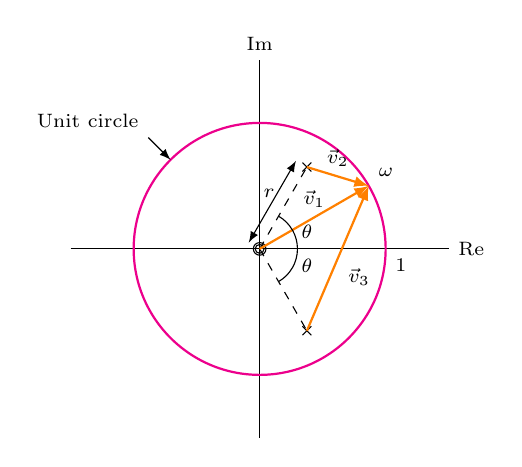
\begin{tikzpicture}[scale=0.8]
    \def\pole{++(135:0.1) -- ++(-45:0.2) ++(135:0.1) -- ++(45:0.1) -- ++(-135:0.2) +(45:0.1)}
    \def\zero{circle (0.1)}

    \draw (-3, 0) -- (3,0) node[anchor=west] {\scriptsize $\mathrm{Re}$};
    \draw (0, -3) -- (0,3) node[anchor=south] {\scriptsize $\mathrm{Im}$};
    %\pause
    \draw[thick, magenta] (0,0) circle (2);
    \draw [latex-] (0,0) ++(135:2) -- ++(135:0.5) node [anchor=south east] {\scriptsize Unit circle};
    \node at (2, 0) [anchor=north west] {\scriptsize $1$};

    %\node at (2, 1) [anchor=west] {\scriptsize $z$-plane};
    \coordinate (p1) at (60:1.5);
    \coordinate (p2) at (-60:1.5);
    \coordinate (o) at (0,0);
    \coordinate (a) at (30:2);
    \draw (p1) node[anchor=north east] {} \pole;
     \draw (p2) node[anchor=north east] {} \pole;
    \draw (0,0) \zero;
    \draw (0,0) circle (0.07);


    \draw[dashed] (o) -- (p1);
    \draw[dashed] (o) -- (p2);
    \draw[-latex, thick, orange] (p1) -- (a) node[black, midway, anchor=south] {\scriptsize $\vec{v}_2$};
  \draw[-latex, thick, orange] (o) -- (a) node[black, midway, anchor=south] {\scriptsize $\vec{v}_1$};
  \draw[-latex, thick, orange] (p2) -- (a) node[black, midway, anchor=north west] {\scriptsize $\vec{v}_3$};

  \draw (0.6,0) arc (0:60:0.6);
  \draw (0.6,0) arc (0:-60:0.6);
  \node at (20:0.8) {\scriptsize $\theta$};
  \node at (-20:0.8) {\scriptsize $\theta$};
   \node at (a) [anchor=south west] {\scriptsize $\omega$};
   
   \draw[latex-latex] (0,0) ++(150:0.2) -- ++(60:1.5) node [midway, black,anchor=east, xshift=0.15cm, yshift=0.1cm] {\scriptsize $r$};

\end{tikzpicture} 